\documentclass[a4paper, 11pt]{article}
\usepackage{geometry}
\geometry{letterpaper, margin=1in}
\usepackage{graphicx}
\graphicspath{ {images/} }

\usepackage{amsmath}
\usepackage{amssymb}  
\usepackage{amsthm}
\usepackage{ulem}

\usepackage{enumitem}


\usepackage{pdfpages} % for including full pdf pages

\usepackage{empheq}

\usepackage{listings}


%format to allow bolded theorems, corollaries, etc...
\newtheorem*{theorem}{Theorem}
\newtheorem*{corollary}{Corollary}
\newtheorem*{lemma}{Lemma}
\newtheorem*{definition}{Definition}
\newtheorem*{Example}{Example} 
\newtheorem*{Remark}{Remark}

% stop typing \mathbb a thousand times 
\newcommand{\R}{\mathbb{R}}
\newcommand{\C}{\mathbb{C}}
\newcommand{\F}{\mathbb{F}}
\newcommand{\E}{\mathcal{E}}
\newcommand{\prob}[2]{\mathcal{P}_{_{#1\rightarrow #2}}}
\newcommand{\M}{\mathbb{M}}
\newcommand{\sphere}{\mathbb{S}}

% commands for bra-ket notation
\newcommand{\bra}[1]{\ensuremath{\left\langle#1\right|}}
\newcommand{\ket}[1]{\ensuremath{\left|#1\right\rangle}}
\newcommand{\bracket}[2]{\ensuremath{\left\langle #1 \middle| #2 \right\rangle}}
\newcommand{\matrixel}[3]{\ensuremath{\left\langle #1 \middle| #2 \middle| #3 \right\rangle}}
\newcommand{\expectation}[1]{\ensuremath{\left\langle #1 \right\rangle}}

% vector stuff
\newcommand{\basis}[1]{\hat{\mathbf{e}}_#1}
\newcommand{\unit}[1]{\hat{\boldsymbol{#1}}}
\newcommand{\bvec}[1]{\vec{\boldsymbol{#1}}}
\newcommand{\threevec}[2]{\begin{pmatrix} #1 \\ #2 \end{pmatrix}}

% change margins for solution
\newenvironment{solution}{%
	\begin{list}{}{%
			\setlength{\topsep}{0pt}%
			\setlength{\leftmargin}{0.5cm}%
			\setlength{\rightmargin}{0.5cm}%
			\setlength{\listparindent}{\parindent}%
			\setlength{\itemindent}{\parindent}%
			\setlength{\parsep}{\parskip}%
		}%
		\item[]}{\end{list}}




\begin{document}
\noindent
\large\textbf{Homework 3} \hfill \textbf{John Waczak} \\
\normalsize PH 653 \hfill  Date: \today \\
Dr. Oksana Ostroverkhova \hfill worked w/ Ryan Tollefsen
\par\noindent\rule{\textwidth}{0.4pt} \\\\



\begin{enumerate}[leftmargin=0em, label=\textbf{\arabic*}]
  \item A hydrogen atom in its ground state is placed in an electric field $\bvec{\E} =
    \bvec{\E_0}\sin\omega t$ of angular frequency $\omega>me^4/2\hbar^3$. In
    this problem, you will investigate the probability of ionizing the hydrogen
    atom. The wavefunctions of the electron in the ionized state may be taken to
    be plane waves.\\

   
  
  \begin{enumerate}[leftmargin=2em, label=(\textbf{\alph*})]
    \item Write down wavefunctions describing the initial and final state.\\
      \begin{solution}
        The initial state is said to be the ground state of the hydrogen atom.
        Therefore, we have
        \begin{align}
          \ket{i} &= \ket{100}  \\
          \Rightarrow \psi_i(r,\theta,\phi) = \psi_{100}(r,\theta,\phi) &= \frac{1}{\sqrt{\pi a_0^3}}e^{-r/a_0}
        \end{align}
        The final state is that of the ionized electron which we are instructed
        to describe via a plane wave (along the z-axis).
        \begin{equation}
          \psi_f = \frac{1}{L^{3/2}}e^{i\bvec{k}\cdot\bvec{r}} = \frac{1}{L^{3/2}}e^{ik_z z}
        \end{equation}

      \end{solution}

    \item Present the perturbation as $V_0\exp(i\omega t)+V_0^*\exp(i\omega t)$.
      Find the time-independent matrix element of the perturbation potential.
      \textit{Hint: direct the wave vector of the free electron along the
        z-axis}. \\
      \begin{solution}
        As we noted last week, the electric field is related to the electric
        potential via $\bvec{E}=-\nabla \Phi$. The potential energy of a charge
        $q$ in such a potential field is given by $V = q\Phi$ and therefore, we
        may identify
        \begin{equation}
          V = q\left( \bvec{\E}_0\cdot \bvec{r} \right)\sin(\omega t)
        \end{equation}
        If we use the exponential representation of the sine function, this
        becomes
        \begin{align}
          V &= q\left( \bvec{\E}_0\cdot\bvec{r} \right)\frac{1}{2i}\left(e^{i\omega t}-e^{-i\omega t}  \right) \\
          &= \left(  q\left( \bvec{\E}_0\cdot\bvec{r} \right)\frac{1}{2i}\right)e^{i\omega t}+ \left( q\left( \bvec{\E}_0\cdot\bvec{r} \right)\frac{1}{2i} \right)^* e^{-i\omega t}
        \end{align}
        
      \end{solution}
      
    \item Find the probability per unit time of ionization with ejection of an
      electron into an element of solid angle $d\Omega_k$. \\
      \begin{solution}
        Fermi's golden rule for transition probabilities give us that
        \begin{align}
          dw_{{}_{i\to f}} = \frac{2\pi}{\hbar}|V_{fi}|^2\rho(E)
        \end{align}
        Therefore, we need to find the matrix element and the density of states.
        Because we are transitioning to a free-particle upon ionizing, the
        density of states may be written as
        \begin{equation}
          \rho(E) = \left(\frac{L}{2\pi}\right)^3\frac{m}{\hbar^2}k_f d\Omega_f
        \end{equation}
        which I will derive in question (2) later. It therefore remains for us
        to calculate this matrix element given by
        \begin{equation}
          V_{fi} = \matrixel{f}{\frac{q\left(\bvec{\E}_0\cdot \bvec{r}\right)}{2}}{i}
        \end{equation}
        where I have suppressed the complex phase because in the end we take the
        squared norm of this matrix element anyways.\\

        We can now expand this in terms of our initial and final states
        \begin{align}
          V_{fi} = \frac{q}{2}\frac{1}{L^{3/2}}\frac{1}{\sqrt{\pi a_0^3}}\int\limits_{\text{all space}}e^{-ik_z z}\left(\bvec{\E}_0\cdot\bvec{r}  \right) e^{-r/a_0}dV
        \end{align}
        We can make two further simplifications before attempt to solve this
        integral. The first is to recognize that $z=r\cos\theta$ in polar
        coordinates. The second is that we can write out the Cartesian dot
        product $\bvec{\E}_0\cdot\bvec{r}$ in spherical coordinates as
        \begin{equation}
          \bvec{\E}_0\cdot\bvec{r} = \E_{0x}r\cos\phi\sin\theta +  \E_{0y}r\sin\phi\sin\theta + \E_{0z}r\cos\theta 
        \end{equation}
        Therefore the full integral may be written as
        \begin{align}
          V_{fi}= \frac{q}{2L^{3/2}\sqrt{\pi a_0^3}}\int\limits_0^\infty\int\limits_0^\pi\int\limits_0^{2\pi}e^{-ik_zr\cos\theta}\Bigg[&\E_{0x}r\cos\phi\sin\theta +\nonumber\\
          &\E_{0y}r\sin\phi\sin\theta +\nonumber\\
            &E_{0z}r\cos\theta \Bigg]e^{-r/a_0}r^2\sin\theta d\phi d\theta dr
        \end{align}
        At this point I used Mathematica to calculate the integral and found
        \begin{figure}[!hbt]
          \centering
          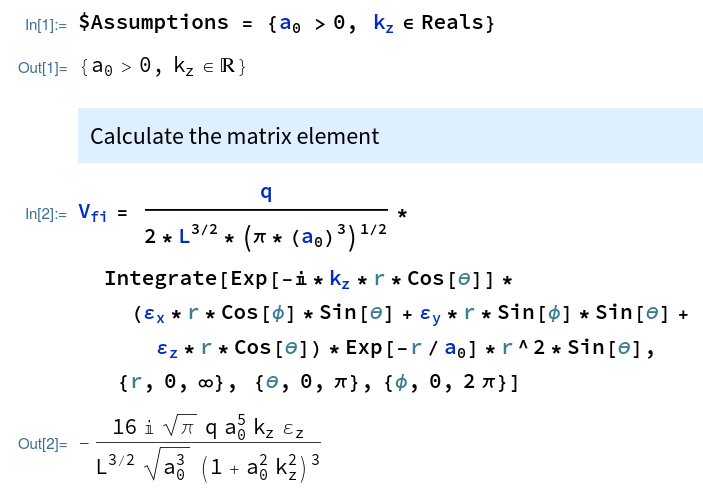
\includegraphics[width=0.8\columnwidth]{integral_1}
        \end{figure}
        \newpage
        so that the matrix element is
        \begin{equation}
          V_{fi} = -\frac{16iq\E_{0z}\sqrt{\pi}}{L^{3/2}}\frac{k_za_0^{7/2}}{(1+k_z^2a_0^2)^3}
        \end{equation}
        Now we have everything needed to write the transition rate 
        \begin{align}
          dw_{{}_{i\to f}} &= \left( \frac{2\pi}{\hbar} \right)\left| V_{fi} \right|^2\rho(E) \\
                          &= \left( \frac{2\pi}{\hbar} \right)\left| -\frac{16iq\E_{0z}\sqrt{\pi}}{L^{3/2}}\frac{k_za_0^{7/2}}{(1+k_z^2a_0^2)^3} \right|^2\rho(E) \\
                          &= \left( \frac{2\pi}{\hbar} \right)\frac{16^2q^2\E_{0z}^2\pi}{L^{3}}\frac{k_z^2a_0^{7}}{(1+k_z^2a_0^2)^^6} \rho(E) \\
                          &= \left( \frac{2\pi}{\hbar} \right)\frac{16^2q^2\E_{0z}^2\pi a^5}{L^{3}}\frac{k_z^2a_0^{2}}{(1+k_z^2a_0^2)^^6} \rho(E) \\
                          &= \left( \frac{2\pi}{\hbar} \right)\frac{16^2q^2\E_{0z}^2\pi a^5}{L^{3}}\frac{k_z^2a_0^{2}}{(1+k_z^2a_0^2)^^6} \left( \frac{L}{2\pi} \right)^3\frac{m}{\hbar^2}k_zd\Omega
        \end{align}
        which simplifies to
        \begin{equation}
          dw = \frac{64\E_{0z}^2a_0^3}{\pi\hbar}\frac{(k_za_0)^3}{(1+k_z^2a_0^2)^6}d\Omega
        \end{equation}
        
          
      \end{solution}
      
      
    \item By integrating over all directions of emission of the electron, find the
      total probability of ionization of the atom. Express it in terms of the Bohr
      radius, electric field amplitude, frequency of the electric field
      oscillation and $\omega_0=E_I/\hbar$, where $E_I$ is the ionization energy
      of the hydrogen atom. Analyze your probability (i.e. get as much physics as
      you can from your expression). Plot it as a function of the frequency
      $\omega$. \\

      \begin{solution}
        Integrating our result from part (c) over all solid angle gives
        \begin{equation}
          w_{{}_{i\to f}} = \frac{256a_0^3\E_{0z}^2}{\hbar}\frac{(k_za_0)^3}{(1+k_z^2a_0^2)^6}
        \end{equation}
        Conservation of energy for absorption gives us that
        \begin{equation}
          \hbar\omega = \frac{\hbar^2k_z^2}{2m}+\hbar\omega_0
        \end{equation}
        so that
        \begin{equation}
          k_z^2 = \frac{2m}{\hbar}(\omega-\omega_0)
        \end{equation}
        furthermore, if we recall that the Bohr radius is defined as
        $a_0=\frac{\hbar^2}{m^2q^2}$ then we can say
        \begin{equation}
          k_z^2a_0^2 = \frac{2m}{\hbar}(\omega-\omega_0)\frac{\hbar^4}{m^4q^4} = \frac{\omega-\omega_0}{\omega_0}
        \end{equation}
        where the frequency corresponding to the ionization energy of hydrogen
        is $\omega_0=\frac{mq^4}{2\hbar^3}$
        therefore, we can conclude that the total transition rate is given by
        \begin{equation}
          w_{{}_{i\to f}}= \frac{256a_0^3\E_{0z}^2a_0^3}{\hbar}\left(\frac{\omega_0}{\omega}\right)^6\left( \frac{\omega}{\omega_0}-1 \right)^{3/2}
        \end{equation}
        A plot of this equation as a function of $\omega$ with everything else
        set to 1 for convenience is shown below.

        \begin{figure}[!hbt]
          \centering
          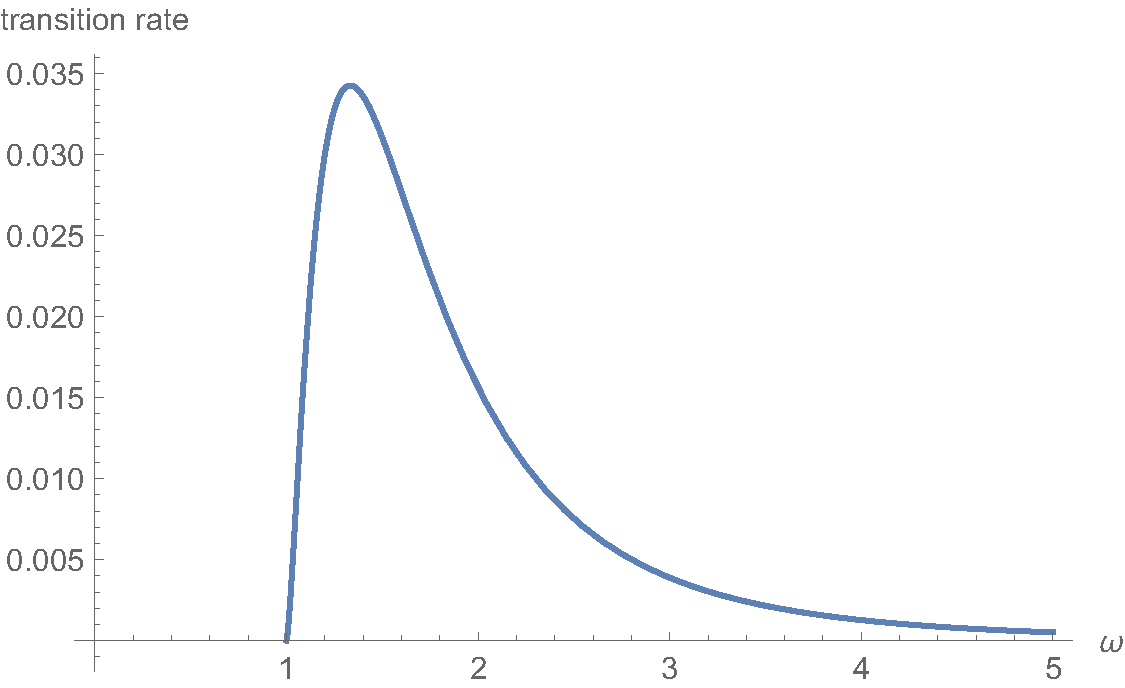
\includegraphics[width=0.75\columnwidth]{transition_rate}
        \end{figure}
        Here we see some interesting physics. First, as we expect, for
        frequencies below $\omega_0$ we do not see ionization. This clearly
        makes sense as the field does not have enough energy to force the
        transition. The biggest surprise is that the maximum (resonance?) does
        not occur when the driving frequency is $\omega=\omega_0$. 

        
      \end{solution}
      
  \end{enumerate}
  
  \item Consider elastic scattering of an electron by a nucleus so that the
    electron-nucleus interaction is treated as a perturbation and is described
    by some potential $V(\bvec{r})$. Use Fermi's golden rule to calculate
    transition rates from some initial state $\ket{i}$ to some final state
    $\ket{f}$. For this, you will need to calculate the matrix element of the
    the perturbation potential and the density of states.\\

    \begin{enumerate}[leftmargin=2em, label=(\textbf{\alph*})]
      \item Write down wavefunctions describing initial and final state of the
        electron. Use plane waves as an approximation for the  wavefunction of
        the electron.\\
        \begin{solution}
          We are considering a scattering problem for which our initial and
          final states may be treated as plane waves. I will use the
          normalization condition used by Sakurai in equation (5.8.27)
          \begin{align}
            \bracket{r}{i} &= \frac{1}{L^{3/2}}e^{i\bvec{k}_i\cdot \bvec{r}} \\
            \bracket{r}{f} &= \frac{1}{L^{3/2}}e^{i\bvec{k}_f\cdot \bvec{r}} \\ 
          \end{align}
          where I have assumed that the electron approaches the nucleus in a
          direction $\bvec{k}_i$ and exits the collision with $\bvec{k}_f$.
          
        \end{solution}
        
      \item Write down the integral you need to solve to find the matrix
        element. Do you see any relation to a Fourier transform?\\
        \begin{solution}
          To find the matrix element, we have to calculate the following
          \begin{align}
            V_{fi} &= \matrixel{f}{V(\bvec{r})}{f} \\
                   &= \frac{1}{L^3}\int\limits_{\text{all space}} e^{-i\bvec{k}_f\cdot\bvec{r}}V(\bvec{r}) e^{i\bvec{k}_i\cdot\bvec{r}}d^3\bvec{r} \\
            &= \frac{1}{L^3}\int\limits_{\text{all space}} V(\bvec{r})e^{i(\bvec{k}_i-\bvec{k}_f)\cdot \bvec{r}}\;d^3\bvec{r} 
          \end{align}
          If we we called $\bvec{k}=\bvec{k}_i-\bvec{k}_f$ then this would look
          just like a Fourier transform of $V(\bvec{r})$ up to the normalization constant. \\
        \end{solution}
        
        
      \item Write down $\rho(E)$. \\
        \begin{solution}
          After scattering, the subsequent plane wave has wave vector
          $\bvec{k}_f$ and therefore, an associated energy
          \begin{equation}
            E_k = \frac{\hbar^2k_f^2}{2m} 
          \end{equation}
          because we are normalizing our plane wave as if it were a particle in
          the box with periodic boundary conditions, we require
          \begin{equation}
            k_f = \frac{2\pi n_f}{L}
          \end{equation}
          so that the energy may be rewritten as
          \begin{equation}
            E = \frac{4\pi^2(n_x^2+n_y^2+n_z^2)\hbar^2}{2mL^2}\equiv \frac{2\pi^2n^2\hbar^2}{mL^2}
          \end{equation}
          Note that I have written $n^2=n_x^2+n_y^2+n_z^2$ i.e. the magnitude of
          this abstract vector in $k$ space. If we allow $L\to\infty$
          then we may effectively treat $n$ as a continuous variable because it
          will always be small as compared with $L$. 

          Now let us consider what happens if this ``vector'' falls in a region
          of length $dn$ and solid angle $d\Omega$. The volume element spanning
          this region in $k$ space is therefore given by $n^2\;dn\;d\Omega$.

          The density of states is a quantity defined such that $\int\rho(E)dE$
          gives the number possible states. We can therefore zap our equation
          for the energies with d to find
          \begin{align}
            dE = \frac{\hbar^2k_f}{m}dk_f = \frac{(2\pi)^2\hbar^2n}{mL^2}dn
          \end{align}
          with this in mind, the number of states in this infinitesimal region
          is given by
          \begin{align}
            n^2\;dn\;d\Omega &= n^2\;d\Omega\frac{dn}{dE}dE \\
                             &= d\Omega\;n^2\frac{mL^2}{(2\pi)^2\hbar^2n}dE \\
                             &= d\Omega\;\frac{mL^2n}{(2\pi)^2\hbar^2}dE \\
                             &= d\Omega\frac{mL^2}{(2\pi)^2\hbar^2}\frac{L}{2\pi}k_f\;dE\\
                             &= \left( \frac{L}{2\pi} \right)^3 \frac{m}{\hbar^2}k_fd\Omega\; dE
          \end{align}
          Therefore, the density of states is just the coefficient of $dE$,
          namely,
          \begin{equation}
            \rho_f(E) = \left( \frac{L}{2\pi} \right)^3 \frac{m}{\hbar^2}k_f d\Omega 
          \end{equation}
          It's cool how we were able to escape the ``particle in a box''
          n dependence and return to the plane wave $k_f$ wavevector. \\

        \end{solution}
        
      \item Combine the results of (b) and (c) into the transition probability
        per unit time and differential cross-section. Discuss how one would
        probe this experimentally. If we want to detect the scattered electron,
        does it matter where the detector is placed?\\
        \begin{solution}
          Fermi's Golden rule dictates that the transition rate is given by
          \begin{equation}
            dw_{{}_{i\rightarrow f}} = \frac{2\pi}{\hbar}|V_{fi}|^2\rho(E)
          \end{equation}
          and therefore, using the previous results, we have that this becomes
          \begin{equation}
            dw_{{}_{i\rightarrow f}} = \frac{2\pi}{\hbar} \left| \frac{1}{L^3}\int\limits_{\text{all space}} V(\bvec{r})e^{i(\bvec{k}_i-\bvec{k}_f)\cdot \bvec{r}}\;d^3\bvec{r}  \right|^2   \left( \frac{L}{2\pi} \right)^3 \frac{m}{\hbar^2}k_f\;d\Omega
          \end{equation}

          Using this, we can define the  cross-section as
          \begin{equation}
            \sigma = \frac{\text{transition rate}}{\text{flux}}
          \end{equation}
          where in this context, the flux can be interpreted as the
          ``probability current'' through the volume of our cube. i.e.
          \begin{equation}
            \frac{v}{L^3}
          \end{equation}
          where $v$ is the electron's speed. Quantum mechanically, the
          particle's momentum is $\hbar k_f$ so that the velocity is just
          \begin{equation}
            v = \frac{\hbar k_f}{m}
          \end{equation}
          Putting this all together yields
          \begin{align}
            \sigma &= \frac{dw}{\frac{\hbar k_f}{mL^3}} = \frac{mL^3}{\hbar k_f}\frac{2\pi}{\hbar} \left| \frac{1}{L^3}\int\limits_{\text{all space}} V(\bvec{r})e^{i(\bvec{k}_i-\bvec{k}_f)\cdot \bvec{r}}\;d^3\bvec{r}  \right|^2   \left( \frac{L}{2\pi} \right)^3 \frac{m}{\hbar^2}k_f\;d\Omega \\
                   &=\frac{m^2}{(2\pi)^2\hbar^4} \left| \int\limits_{\text{all space}} V(\bvec{r})e^{i(\bvec{k}_i-\bvec{k}_f)\cdot \bvec{r}}\;d^3\bvec{r}  \right|^2 \;d\Omega
          \end{align}
          Note that the volume $L^3$ has disappeared from the equation! From
          this, the differential cross section is given by
          
          \begin{equation}
            \frac{d\sigma}{d\Omega} = \frac{m^2}{(2\pi)^2\hbar^4} \left| \int\limits_{\text{all space}} V(\bvec{r})e^{i(\bvec{k}_i-\bvec{k}_f)\cdot \bvec{r}}\;d^3\bvec{r}  \right|^2 
          \end{equation}
          To probe this experimentally, we would fire an electron beam at a
          neutral atom, varying the impact parameter $b$ in order to learn about
          the properties of the potential $V(\bvec{r})$. For neutral atoms, we
          would expect the potential to be spherically symmetric as we assumed
          above. Where we place the detector with respect to the atom and
          electron beam is important because moving the detector checks the
          angular dependence of the differential cross section. For elastic
          collisions, we should expect some kind symmetric angular dependence in
          the plane perpendicular to the electron beam as illustrated in the
          following figure:
          \begin{figure}[!hbt]
            \centering
            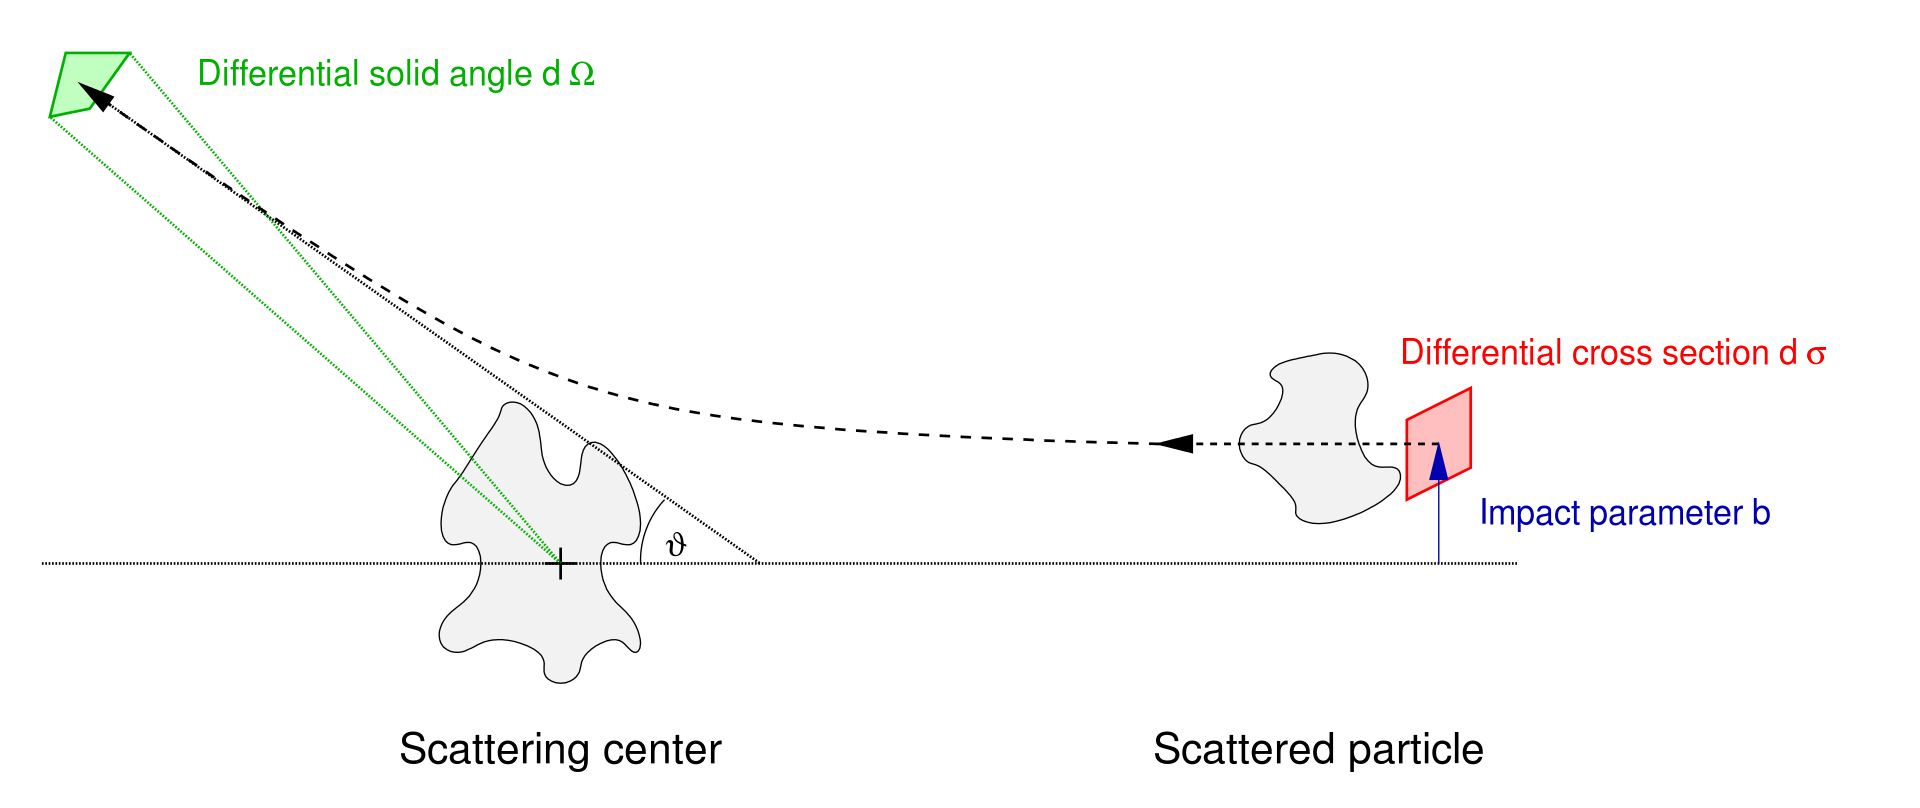
\includegraphics[width=0.6\columnwidth]{cross_section}
          \end{figure}
          
            
        \end{solution}
        
    \end{enumerate}
      
    
  
\end{enumerate}

  
\end{document}






























